\documentclass{article}
\usepackage[utf8]{inputenc}
\usepackage{geometry}
\geometry{a4paper, margin=2.54cm}
\usepackage{amsmath}
\usepackage{amsfonts}
\usepackage{amssymb}
\usepackage{graphicx}
\usepackage{enumitem}
\usepackage{xcolor}
\usepackage{pgfgantt}
\usepackage{booktabs}
\usepackage{array}
\usepackage{tikz}
\usetikzlibrary{shapes.geometric, arrows.meta, positioning}

\title{Project-X: Agent Development Guidance}
\author{Alberto Espinosa\\
KSquare Group}
\date{July 21, 2025}

\begin{document}

\maketitle

This document provides detailed guidance for the Project-X team to develop the eight agents constituting the MVP of the agent-based architecture. Each agent is designed to operate within a LangGraph environment, leveraging pre-trained Ollama models. The descriptions include the agent’s role, goal, inputs, outputs, and recommendations for configuring Ollama parameters and crafting effective prompts. A general agent structure is also provided to ensure seamless integration into the LangGraph pipeline.

\section{Agent Architecture Overview}

Each agent is a modular component in a LangGraph workflow, processing inputs from the previous agent (or user) and producing outputs for the next. Agents use pre-trained Ollama models for natural language processing tasks, such as prompt parsing or result interpretation, and Python libraries (e.g., \texttt{faker}, \texttt{scipy}, \texttt{pycaret}) for data-related tasks. The general structure of an agent is illustrated below, designed for integration into LangGraph’s graph-based execution.

\begin{figure}[h]
\centering
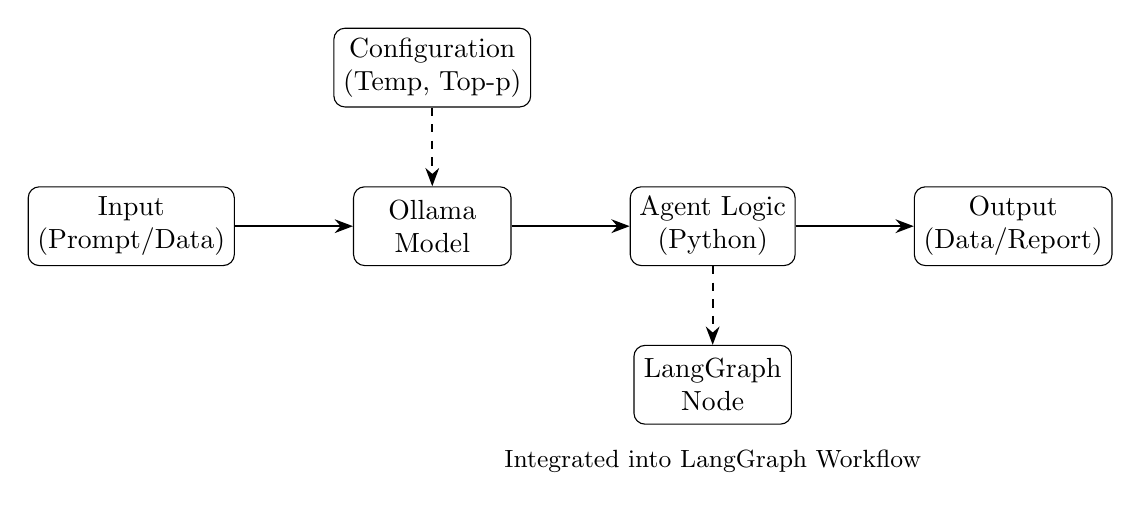
\begin{tikzpicture}[
    box/.style={rectangle, draw, rounded corners, minimum height=1cm, minimum width=2cm, align=center},
    arrow/.style={-Stealth, thick}
]
\node[box] (input) {Input\\(Prompt/Data)};
\node[box, right=1.5cm of input] (ollama) {Ollama\\Model};
\node[box, right=1.5cm of ollama] (logic) {Agent Logic\\(Python)};
\node[box, right=1.5cm of logic] (output) {Output\\(Data/Report)};
\node[box, above=1cm of ollama] (config) {Configuration\\(Temp, Top-p)};
\node[box, below=1cm of logic] (langgraph) {LangGraph\\Node};
\draw[arrow] (input) -- (ollama);
\draw[arrow] (ollama) -- (logic);
\draw[arrow] (logic) -- (output);
\draw[arrow, dashed] (config) -- (ollama);
\draw[arrow, dashed] (logic) -- (langgraph);
\node[below=0.2cm of langgraph] {\small Integrated into LangGraph Workflow};
\end{tikzpicture}
\caption{General Agent Structure}
\end{figure}

Each agent receives input (e.g., user prompt, dataset, or previous agent’s output), processes it using an Ollama model (for NLP tasks) and Python logic (for data tasks), and produces structured output for the next agent. Configuration parameters (temperature, top-p) are set to balance creativity and determinism. The agent is encapsulated as a LangGraph node, enabling sequential execution and state management.

\section{Agent Descriptions}

\subsection{User Prompt Parser Agent}

\textbf{Role}: Parses user-provided prompts describing datasets or problem statements into structured inputs for downstream agents.

\textbf{Goal}: Convert natural language prompts into a JSON object specifying dataset characteristics or problem details, ensuring compatibility with the Code Generation for Synthetic Data Agent.

\textbf{Inputs}:
\begin{itemize}[label=--]
    \item \textbf{Source}: User-provided text prompt (e.g., “Create a dataset for fraud detection with columns: transaction\_id (int), amount (float), country (string), is\_fraud (bool)”).
    \item \textbf{Format}: Plain text string.
    \item \textbf{Handling}: The agent uses an Ollama model to extract key details (e.g., column names, types, target variable) and validates the prompt for completeness (e.g., presence of a target variable).
\end{itemize}

\textbf{Outputs}:
\begin{itemize}[label=--]
    \item \textbf{Format}: JSON object, e.g., \texttt{\{"columns": [\{"name": "transaction\_id", "type": "int"\}, \{"name": "amount", "type": "float"\}, \{"name": "country", "type": "string"\}, \{"name": "is\_fraud", "type": "bool"\}], "target": "is\_fraud", "rows": 1000\}}.
    \item \textbf{Usability}: Structured JSON ensures the Code Generation Agent can directly interpret column types and generate appropriate code. The output includes a default row count (e.g., 1000) if unspecified.
\end{itemize}

\textbf{Ollama Configuration}:
\begin{itemize}[label=--]
    \item \textbf{Temperature}: 0.3 (low to ensure deterministic parsing of structured information).
    \item \textbf{Top-p}: 0.9 (high to allow slight flexibility in interpreting varied prompt phrasings).
\end{itemize}

\textbf{Prompt Engineering Suggestions}:
\begin{itemize}[label=--]
    \item Use a clear instruction: “Extract dataset details (column names, types, target variable, row count) from the following prompt and output as JSON. If row count is missing, default to 1000.”
    \item Provide examples in the prompt: “Example input: ‘Dataset with user\_id (int), purchase (float), date (string), churn (bool).’ Example output: \texttt{\{"columns": [...], "target": "churn", "rows": 1000\}}.”
    \item Include error handling: “If the prompt lacks a target variable, return an error message requesting clarification.”
\end{itemize}

\subsection{Code Generation for Synthetic Data Agent}

\textbf{Role}: Generates Python code to create synthetic datasets based on user specifications, ensuring well-formed data for downstream agents.

\textbf{Goal}: Produce executable Python code using \texttt{faker} for tabular data or \texttt{scipy} for time series, tailored to the dataset description.

\textbf{Inputs}:
\begin{itemize}[label=--]
    \item \textbf{Source}: JSON object from the User Prompt Parser Agent.
    \item \textbf{Format}: JSON, e.g., \texttt{\{"columns": [\{"name": "transaction\_id", "type": "int"\}, ...], "target": "is\_fraud", "rows": 1000\}}.
    \item \textbf{Handling}: The agent interprets the JSON to select the appropriate library (\texttt{faker} for tabular, \texttt{scipy} for time series based on keywords like “date” or “timestamp”) and validates column types.
\end{itemize}

\textbf{Outputs}:
\begin{itemize}[label=--]
    \item \textbf{Format}: CSV file containing the synthetic dataset, e.g., \texttt{data.csv} with columns \texttt{transaction\_id, amount, country, is\_fraud}.
    \item \textbf{Usability}: The CSV is directly usable by the EDA Agent, with standard data types (int, float, string, bool) and a target column for PyCaret compatibility.
\end{itemize}

\textbf{Ollama Configuration}:
\begin{itemize}[label=--]
    \item \textbf{Temperature}: 0.5 (moderate to balance code accuracy with flexibility for library selection).
    \item \textbf{Top-p}: 0.85 (moderate to ensure relevant code snippets).
\end{itemize}

\textbf{Prompt Engineering Suggestions}:
\begin{itemize}[label=--]
    \item Use a directive: “Generate Python code to create a synthetic dataset based on the provided JSON. Use \texttt{faker} for tabular data or \texttt{scipy} for time series if ‘date’ or ‘timestamp’ is present.”
    \item Include examples: “For \texttt{\{"columns": [\{"name": "id", "type": "int"\}, \{"name": "date", "type": "string"\}]\}}, output code using \texttt{scipy} to generate time series.”
    \item Specify validation: “Ensure the code produces a CSV with the exact column names and types specified.”
\end{itemize}

\subsection{EDA Agent}

\textbf{Role}: Conducts non-traditional exploratory data analysis to produce a detailed dataset description, assessing its suitability for the problem.

\textbf{Goal}: Generate a structured report on dataset characteristics, focusing on data types, target variable suitability, and domain relevance, without classical statistics.

\textbf{Inputs}:
\begin{itemize}[label=--]
    \item \textbf{Source}: CSV dataset from the Code Generation Agent or user-provided.
    \item \textbf{Format}: CSV file, e.g., \texttt{data.csv} with columns \texttt{transaction\_id, amount, country, is\_fraud}.
    \item \textbf{Handling}: The agent uses Python (e.g., \texttt{pandas}) to analyse column types, target variable distribution, and domain-specific patterns (e.g., country diversity for fraud detection).
\end{itemize}

\textbf{Outputs}:
\begin{itemize}[label=--]
    \item \textbf{Format}: JSON report, e.g., \texttt{\{"columns": [\{"name": "amount", "type": "float", "relevance": "high for fraud detection"\}], "target\_suitable": true, "notes": "Diverse countries enhance fraud detection"\}}.
    \item \textbf{Usability}: The JSON report is consumable by the PyCaret Model Running Agent, providing context for model selection (e.g., classification for boolean targets).
\end{itemize}

\textbf{Ollama Configuration}:
\begin{itemize}[label=--]
    \item \textbf{Temperature}: 0.4 (low to ensure precise analysis).
    \item \textbf{Top-p}: 0.9 (high to allow nuanced descriptions of dataset value).
\end{itemize}

\textbf{Prompt Engineering Suggestions}:
\begin{itemize}[label=--]
    \item Use a clear task: “Analyse the CSV dataset and produce a JSON report describing column types, target variable suitability, and domain relevance. Avoid statistical metrics like correlations.”
    \item Provide context: “For fraud detection, assess if columns like ‘country’ or ‘amount’ are relevant.”
    \item Include examples: “Output example: \texttt{\{"columns": [...], "target\_suitable": true, "notes": "Sufficient samples for classification"\}}.”
\end{itemize}

\subsection{PyCaret Model Running Agent}

\textbf{Role}: Generates and executes PyCaret code to train a machine learning model, saving the model and its performance metrics/plots.

\textbf{Goal}: Automate model training for classification or regression tasks, storing the model and evaluation outputs for interpretation.

\textbf{Inputs}:
\begin{itemize}[label=--]
    \item \textbf{Source}: CSV dataset from the EDA Agent and JSON report from the EDA Agent.
    \item \textbf{Format}: CSV (e.g., \texttt{data.csv}) and JSON (e.g., \texttt{\{"target": "is\_fraud"\}}).
    \item \textbf{Handling}: The agent uses the JSON to identify the target variable and problem type (e.g., classification), then runs PyCaret’s \texttt{setup} and \texttt{compare\_models}.
\end{itemize}

\textbf{Outputs}:
\begin{itemize}[label=--]
    \item \textbf{Format}: Saved model file (e.g., \texttt{model.pkl}), metrics JSON (e.g., \texttt{\{"accuracy": 0.85, "auc": 0.90\}}), and plots (e.g., \texttt{confusion\_matrix.png}).
    \item \textbf{Usability}: The model and metrics are directly usable by the Model and Results Interpreter Agent for performance analysis.
\end{itemize}

\textbf{Ollama Configuration}:
\begin{itemize}[label=--]
    \item \textbf{Temperature}: 0.3 (low for precise code generation).
    \item \textbf{Top-p}: 0.8 (moderate to ensure standard PyCaret code).
\end{itemize}

\textbf{Prompt Engineering Suggestions}:
\begin{itemize}[label=--]
    \item Use a directive: “Generate PyCaret code to train a model on the provided CSV, using the target variable from the JSON. Save the model and metrics/plots.”
    \item Include examples: “For \texttt{\{"target": "is\_fraud"\}}, use \texttt{setup(data, target='is\_fraud', session\_id=123)}.”
    \item Specify outputs: “Save the model as \texttt{model.pkl}, metrics as JSON, and plots as PNG files.”
\end{itemize}

\subsection{Model and Results Interpreter Agent}

\textbf{Role}: Interprets PyCaret model metrics and plots, generating a context-specific performance report.

\textbf{Goal}: Provide a clear explanation of model performance (e.g., accuracy, AUC) in the context of the problem (e.g., fraud detection), combining model and pipeline insights.

\textbf{Inputs}:
\begin{itemize}[label=--]
    \item \textbf{Source}: Metrics JSON, plots, and CSV dataset from the PyCaret Model Running Agent; JSON report from the EDA Agent.
    \item \textbf{Format}: JSON (e.g., \texttt{\{"accuracy": 0.85\}}), PNG files, CSV, and EDA JSON.
    \item \textbf{Handling}: The agent uses Ollama to interpret metrics and plots, contextualising them with the EDA report (e.g., “High recall suitable for fraud detection”).
\end{itemize}

\textbf{Outputs}:
\begin{itemize}[label=--]
    \item \textbf{Format}: JSON report, e.g., \texttt{\{"performance": "Accuracy: 0.85, suitable for fraud detection due to balanced dataset", "recommendations": "Increase recall for stricter flagging"\}}.
    \item \textbf{Usability}: The report is consumable by the Report Formatter Agent for final output.
\end{itemize}

\textbf{Ollama Configuration}:
\begin{itemize}[label=--]
    \item \textbf{Temperature}: 0.6 (moderate to allow interpretive flexibility).
    \item \textbf{Top-p}: 0.9 (high to capture nuanced explanations).
\end{itemize}

\textbf{Prompt Engineering Suggestions}:
\begin{itemize}[label=--]
    \item Use a clear instruction: “Interpret the provided model metrics and plots, using the EDA report for context. Output a JSON report with performance summary and recommendations.”
    \item Provide examples: “For \texttt{\{"accuracy": 0.85\}}, output: \texttt{\{"performance": "High accuracy indicates robust model"\}}.”
    \item Include context: “For fraud detection, prioritise recall over precision.”
\end{itemize}

\subsection{Business Rule Agent}

\textbf{Role}: Applies and interprets business rules on the dataset, producing a modified dataset and rule summary.

\textbf{Goal}: Formalise and apply business rules (e.g., “Flag transactions from country X as suspicious”) and describe their impact in the problem context.

\textbf{Inputs}:
\begin{itemize}[label=--]
    \item \textbf{Source}: CSV dataset from the PyCaret Model Running Agent and a rule prompt from the user.
    \item \textbf{Format}: CSV (e.g., \texttt{data.csv}) and text prompt (e.g., “Flag transactions where country in [‘X’, ‘Y’] as suspicious”).
    \item \textbf{Handling}: The agent formalises the rule into Python code (e.g., \texttt{df['suspicious'] = df['country'].isin(['X', 'Y'])}) and applies it.
\end{itemize}

\textbf{Outputs}:
\begin{itemize}[label=--]
    \item \textbf{Format}: Modified CSV (e.g., \texttt{data\_ruled.csv} with new column \texttt{suspicious}) and JSON rule summary (e.g., \texttt{\{"rule": "Flag countries X, Y", "impact": "10\% transactions flagged"\}}).
    \item \textbf{Usability}: The modified CSV and summary are usable by the Report Formatter Agent.
\end{itemize}

\textbf{Ollama Configuration}:
\begin{itemize}[label=--]
    \item \textbf{Temperature}: 0.4 (low for precise rule formalisation).
    \item \textbf{Top-p}: 0.85 (moderate to ensure accurate code generation).
\end{itemize}

\textbf{Prompt Engineering Suggestions}:
\begin{itemize}[label=--]
    \item Use a directive: “Formalise the provided rule prompt into Python code and apply it to the CSV. Output the modified CSV and a JSON summary of the rule’s impact.”
    \item Include examples: “For ‘Flag amount > 1000’, output code: \texttt{df['flag'] = df['amount'] > 1000}.”
    \item Specify validation: “Ensure the rule is applied to all rows and the summary includes affected row percentage.”
\end{itemize}

\subsection{Configuration Agent}

\textbf{Role}: Allows users to adjust parameters for model training or rule application via a text-based interface.

\textbf{Goal}: Provide a simple mechanism to update configurations (e.g., PyCaret model type, rule thresholds) for flexibility in the pipeline.

\textbf{Inputs}:
\begin{itemize}[label=--]
    \item \textbf{Source}: User-provided configuration prompt.
    \item \textbf{Format}: Text, e.g., “Use random forest for PyCaret” or “Set fraud threshold to 500”.
    \item \textbf{Handling}: The agent parses the prompt to generate a configuration JSON, validating for supported options (e.g., PyCaret algorithms).
\end{itemize}

\textbf{Outputs}:
\begin{itemize}[label=--]
    \item \textbf{Format}: JSON configuration, e.g., \texttt{\{"pycaret\_model": "rf", "fraud\_threshold": 500\}}.
    \item \textbf{Usability}: The JSON is usable by the PyCaret Model Running or Business Rule Agent to adjust their behaviour.
\end{itemize}

\textbf{Ollama Configuration}:
\begin{itemize}[label=--]
    \item \textbf{Temperature}: 0.3 (low for precise parsing).
    \item \textbf{Top-p}: 0.8 (moderate to ensure valid configurations).
\end{itemize}

\textbf{Prompt Engineering Suggestions}:
\begin{itemize}[label=--]
    \item Use a clear task: “Parse the configuration prompt and output a JSON with supported parameters for PyCaret or business rules.”
    \item Provide examples: “For ‘Use random forest’, output: \texttt{\{"pycaret\_model": "rf"\}}.”
    \item Include validation: “Reject unsupported parameters and request clarification.”
\end{itemize}

\subsection{Report Formatter Agent}

\textbf{Role}: Standardises outputs from the pipeline into a unified format for API delivery.

\textbf{Goal}: Combine EDA, model performance, and rule application outputs into a cohesive report, suitable for API integration.

\textbf{Inputs}:
\begin{itemize}[label=--]
    \item \textbf{Source}: JSON reports from EDA, Model and Results Interpreter, and Business Rule Agents; CSV from Business Rule Agent.
    \item \textbf{Format}: Multiple JSON files and CSV.
    \item \textbf{Handling}: The agent aggregates inputs into a single structured output, ensuring consistency.
\end{itemize}

\textbf{Outputs}:
\begin{itemize}[label=--]
    \item \textbf{Format}: JSON report, e.g., \texttt{\{"eda": \{...\}, "model": \{...\}, "rules": \{...\}, "summary": "Model and rules suitable for fraud detection"\}}.
    \item \textbf{Usability}: The JSON is ready for API delivery, ensuring compatibility with Week 6’s API Design and Test phase.
\end{itemize}

\textbf{Ollama Configuration}:
\begin{itemize}[label=--]
    \item \textbf{Temperature}: 0.5 (moderate for clear summarisation).
    \item \textbf{Top-p}: 0.9 (high for comprehensive reporting).
\end{itemize}

\textbf{Prompt Engineering Suggestions}:
\begin{itemize}[label=--]
    \item Use a directive: “Combine the provided JSON reports and CSV into a unified JSON report, summarising key findings.”
    \item Include examples: “Merge \texttt{\{"eda": \{...\}, "model": \{...\}\}} into a single JSON with a summary field.”
    \item Specify format: “Ensure the output is API-compatible JSON with clear sections.”
\end{itemize}

\section{Team Composition}

\begin{table}[h]
\centering
\begin{tabular}{|>{\raggedright\arraybackslash}p{0.2\textwidth}|>{\raggedright\arraybackslash}p{0.3\textwidth}|>{\raggedright\arraybackslash}p{0.2\textwidth}|>{\raggedright\arraybackslash}p{0.3\textwidth}|}
\hline
\textbf{Name} & \textbf{Role} & \textbf{Agent} & \textbf{Comments} \\ \hline
Rafael & ML and APIs for Models, AI-Dev & *** &  \\ \hline
Andrés & Frontend, AI-Dev & *** &  \\ \hline
Carlos & Frontend, AI-Dev & *** & Integrator \\ \hline
Mauricio & Backend, AI-Dev & *** &  \\ \hline
Johnattan & DevOps, AI-Dev & *** &  \\ \hline
Gastón & Tech Lead, AI-Dev & *** &  \\ \hline
Jan & AI--developer & *** &  \\ \hline
Enrique & AI--developer & *** &  \\ \hline
\end{tabular}
\caption{Team Members and Assigned Agents}
\end{table}

\end{document}
